\section{A Silly Idea}
    
    \frame{\sectionpage}
    
    \begin{frame}{Ordinary Differential Equations}
        \uncover<+->{\begin{equation*}
            \dv{x} y(x) + \frac{1}{CR} y(x) = 0
        \end{equation*}}
        
        \uncover<+->{\begin{equation*}
            \dv[2]{x} y(x) + \gamma \dv{x} y(x) + \omega_0^2 y(x) = f(x)
        \end{equation*}}
    \end{frame}
    
    \begin{frame}{Livin' La Vida Loca}
        \uncover<+>{\begin{equation*}
            \dv[2]{x} y(x) + \gamma \dv{x} y(x) + \omega_0^2 y(x) = f(x)
        \end{equation*}}
        \uncover<+>{\[ \Downarrow \]
        \begin{equation*}
            \colch{\dv[2]{x} + \gamma \dv{x} + \omega_0^2} y(x) = f(x)
        \end{equation*}}
        \uncover<+>{\[ \Downarrow \]
        \begin{equation*}
            y(x) = \frac{f(x)}{\dv[2]{x} + \gamma \dv{x} + \omega_0^2}
        \end{equation*}}
    \end{frame}
    
    \begin{frame}{Livin' La Vida Loca}
        \centering
        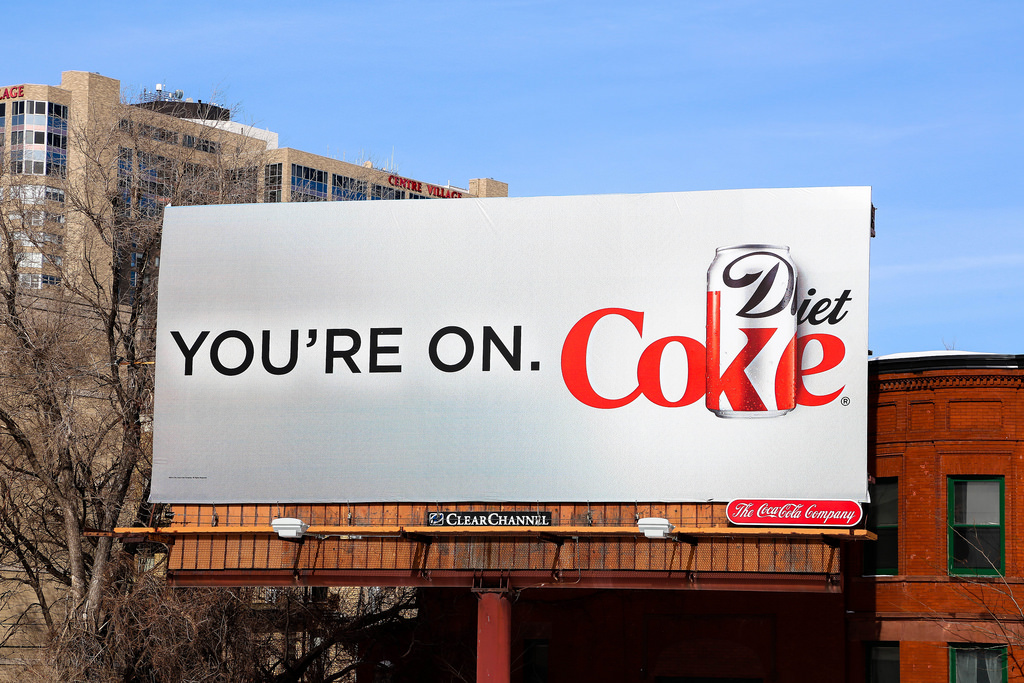
\includegraphics[width = 0.8\textwidth]{images/coke.jpg}
    \end{frame}
    
    \begin{frame}{Pandora's Box}
        \centering
        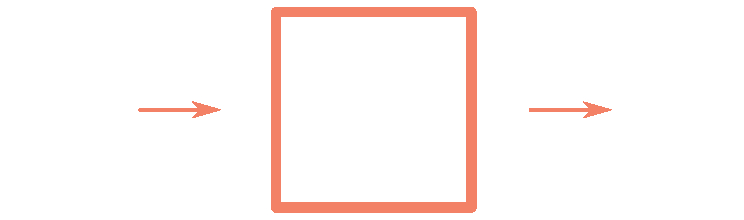
\includegraphics[width = 0.9\textwidth]{images/fourier-1.pdf}
    \end{frame}
    
    \begin{frame}{Pandora's Box}
        \centering
        
\includegraphics[width = 0.9\textwidth]{images/fourier-2.pdf}
    \end{frame}
    
    \begin{frame}{Pandora's Box}
        \centering
        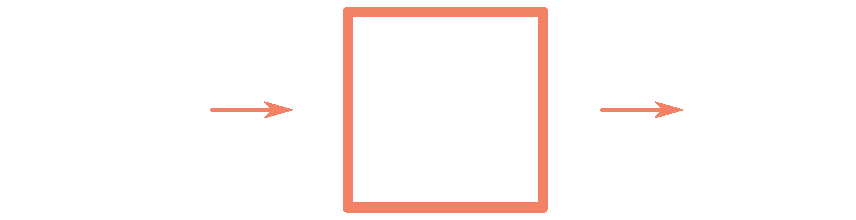
\includegraphics[width = 0.9\textwidth]{images/fourier-3.pdf}
    \end{frame}
    
    \begin{frame}{Pandora's Box}
        \centering
        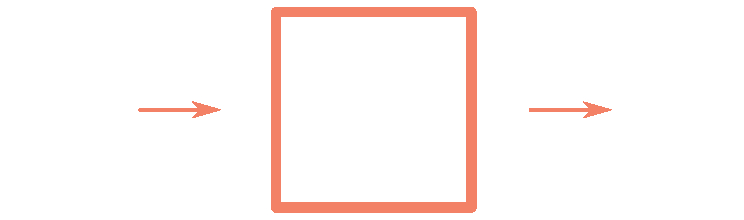
\includegraphics[width = 0.9\textwidth]{images/fourier-4.pdf}
    \end{frame}
    
    \begin{frame}{Pandora's Box}
        \centering
        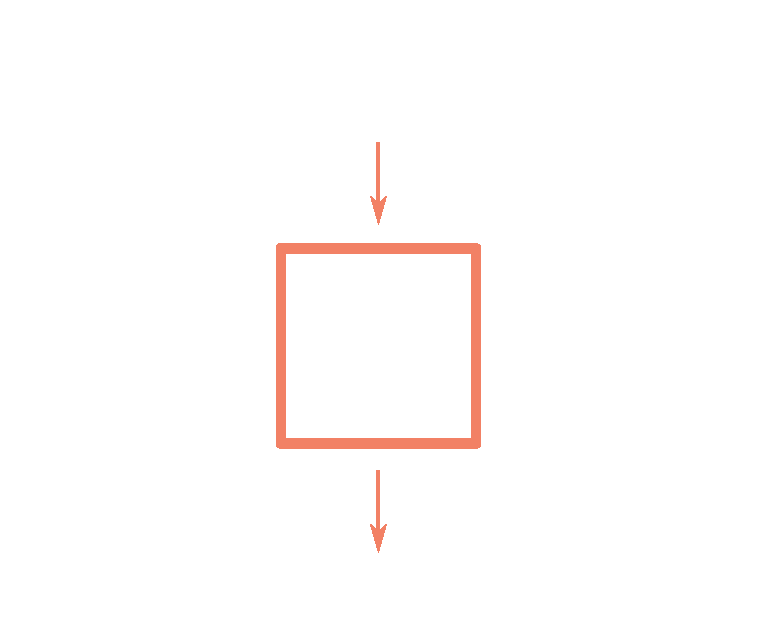
\includegraphics[height = 0.7\textheight]{images/fourier-5.pdf}
    \end{frame}
    
    \begin{frame}{Box Proposal}
        \uncover<+>{\begin{equation*}
            \mathcal{F}[f](\xi) = \hat{f}(\xi) = \frac{1}{\sqrt{2\pi}} \int_{-\infty}^{+\infty} f(x) e^{-i x \xi} \dd{x}
        \end{equation*}}
        \uncover<+>{\begin{equation*}
            \mathcal{F}^{-1}[\hat{f}](x) = f(x) = \frac{1}{\sqrt{2\pi}} \int_{-\infty}^{+\infty} \hat{f}(\xi) e^{i x \xi} \dd{\xi}
        \end{equation*}}
    \end{frame}
    
    \begin{frame}{Quality Control}
        \uncover<+>{\begin{equation*}
            \widehat{(f + \alpha g)}(\xi) = \frac{1}{\sqrt{2\pi}} \int_{-\infty}^{+\infty} \prnt{f(x) + \alpha g(x)} e^{-i x \xi} \dd{x}
        \end{equation*}}
        \uncover<+>{\[ \Downarrow \]
        \begin{equation*}
            \widehat{(f + \alpha g)}(\xi) = \frac{1}{\sqrt{2\pi}} \int_{-\infty}^{+\infty} f(x) e^{-i x \xi} \dd{x} + \frac{\alpha}{\sqrt{2\pi}} \int_{-\infty}^{+\infty} g(x) e^{-i x \xi} \dd{x}
        \end{equation*}}
        \uncover<+>{\[ \Downarrow \]
        \begin{equation*}
            \widehat{(f + \alpha g)}(\xi) = \hat{f}(\xi) + \alpha \hat{g}(\xi)
        \end{equation*}}
    \end{frame}
    
    \begin{frame}{Quality Control}
        \uncover<+>{\begin{equation*}
            \widehat{f'}(\xi) = \frac{1}{\sqrt{2\pi}} \int_{-\infty}^{+\infty} f'(x) e^{-i x \xi} \dd{x}
        \end{equation*}}
        \uncover<+>{\[ \Downarrow \]
        \begin{equation*}
            \widehat{f'}(\xi) = \eval{\frac{f(x) e^{-ix\xi}}{\sqrt{2\pi}}}^{+\infty}_{-\infty} + i\xi \cdot \frac{1}{\sqrt{2\pi}} \int_{-\infty}^{+\infty} f(x) e^{-i x \xi} \dd{x}
        \end{equation*}}
        \uncover<+>{\[ \Downarrow \]
        \begin{equation*}
            \widehat{f'}(\xi) = i\xi \widehat{f}(\xi)
        \end{equation*}}
    \end{frame}
    
    \begin{frame}{Quality Control}
        \centering
        \huge{The inverse does work}
        
        \normalsize{for appropriate functions}
        
        \tiny{and, sometimes, the Fourier Transform of a function is not in the same set as the original function, but let's forget about this since we do not know a decent theory of integration}
    \end{frame}